\section{Experiment and Evaluation}
In this section we reiterate the problem, provide more detail about the experiment and evaluation process, and describe the system and the data we collected from it to perform the study.


\subsection{Objectives}
The questions we seek the answer(s) for are as follows:


\textsc{RQ 1) Can existing multivariate time series CPD algorithms be used to detect state changes?}


\textsc{RQ 2) How does our approach compare to similar approaches with classical machine learning algorithms (as opposed to deep learning algorithms)?}


\textsc{RQ 3) How does our approach compare to other algorithms?}


\subsection{Metrics}
% To have a quantitative analysis of the algorithms we measure the following metrics.

Our model combines two tasks, finding when a state transition has happened and finding what the new state is. Traditional state models such as EFSMs do not take time (\textit{when} the transition happens) into account. They focus on finding the right invariants and state transitions (\textit{what} the new state should be).

In time series segmentation literature however, the focus is primarily on answering the \textit{when} question rather than the \textit{what}. Since our model tries to answer both, we need metrics that accommodate both.

In CPD-natured tasks there is an inherent class imbalance.
There are far more points where a change has not happened, so the sheer number of true negatives makes metrics such as accuracy almost useless. 
A trivial model can always output 0 (no change) and have an accuracy of 99\% on a input of length 1000 with 10 true change points.
To address this problem, metrics such as precision and recall that do not account for true negatives are used. \cite{Truong2018ChangePointSurvey, Lee2018TimeSeriesSegmentation} 
Precision and recall for that trivial model will be 0 better reflecting its poor performance.


\subsubsection{Modified F1-Score}
F1-Score the harmonic mean of precision and recall. 
To define precision and recall we need to define true positive, false positive, and false negative first.
Similar to \cite{Lee2018TimeSeriesSegmentation} and \cite{Truong2018ChangePointSurvey}, we use a tolerance margin $\tau$, and if a detected state transition ($\in \hat{CP}_k$) is within $\pm\tau$ of a true transition that is a true positive. 
This tolerance covers the \textit{when}, to take the \textit{what} into the frame we use a parameter $0 \leq \alpha < 1$ that penalizes detecting transitions at a correct time but to an incorrect state.

\begin{equation} \label{eq:cp_hat}
\hat{CP}_k = \big\{(t, \hat{o}_t)\: |\: \hat{o}_t \neq \hat{o}_{t-1} \big\}
\end{equation}

Please note that in \eqref{eq:cp_hat}, $\hat{o}_t$ refers to $t$th element of output vector $\hat{O}$, as previously defined in \eqref{eq:model_as_function}.

\begin{equation}
TP =\sum_{(\hat{t}, \hat{s}_t) \in \hat{CP}_k} \mathcal{TP}(\hat{t}, \hat{s}_t)
\end{equation}
\begin{equation*}
\mathcal{TP}(\hat{t}, \hat{s}_t) =
     \begin{cases}
       1      &\quad \exists\: (t, s_t) \in CP_k \;\text{s.t.}\; |t - \hat{t}| < \tau \land s_t = \hat{s}_t \\
       \alpha &\quad \exists\: (t, s_t) \in CP_k \;\text{s.t.}\; |t - \hat{t}| < \tau \land s_t \neq \hat{s}_t  \\
       0     &\quad\text{otherwise.} \\ 
     \end{cases}
\end{equation*}

Similarly we can define false positive and false negative:

\begin{equation} \label{eq:false_negative}
\begin{split}
FP ={}&{}\Big|\big\{ (\hat{t}, \hat{s}_t) \in \hat{CP}_k \;\big|\; \nexists\: (t, s_t) \in CP_k \;\text{s.t.}\; |t - \hat{t}| < \tau\big\}\Big| \\
FN ={}&{}\Big|\big\{ (t, s_t) \in CP_k \;\big|\; \nexists\: (\hat{t}, \hat{s}_t) \in \hat{CP}_k \;\text{s.t.}\; |t - \hat{t}| < \tau\big\}\Big| 
\end{split}
\end{equation}

\subsubsection{Model Fitting Time}


\subsection{Baseline Algorithms}
\subsubsection{CPD algorithms}
A hypothesis is that existing multivariate time series CPD algorithms can be used to solve the problem we are trying to tackle if CPD algorithms would be able to reliably mark the time that state changes happen.
These two steps are our proposed approach of doing that:
1) Applying CPD algorithms to find the time when hidden internal state transitions happen. 
2) Using the state transitions as `events' to form the input of EFSM inference algorithms.

\subsubsection{Classical Machine Learning}
A sliding window of size 10 was rolled over the 10 time series and then flattened to make a vector of size 100 as the input dimensions.


. They performed poorly mainly because they don't have a `memory' as LSTM/GRU neural networks do\\
. The training/prediction performance (time) was not good either ($O(n^4)$)\\


\subsubsection{Deep Learning}

\subsection{Evaluation}


The data was randomly split into two chunks of 95\% and 5\% for training and evaluation.
Adam optimizer \cite{kingma2014adam} was used to optimizer a dice overlap loss function \cite{milletari2016v} in the training process.


\subsection{Experiment Environment}
Training and evaluation was done on a single node running Ubuntu 18.04 LTS (Linux 5.3.0) equipped with Intel Core i7-9700K CPU, 32 gigabytes of main memory and 8 gigabytes of GPU memory on a NVIDIA GeForce RTX 2080 graphics card.
The code was written using TensorFlow 2's keras API.



\subsection{System Under Study} \label{mp_data_collection}

Our case study was a real-time controller system, an AutoPilot developed by Winnipeg based Micro Pilot Inc. Micro Pilot is the world-leader in professional UAV AutoPilot which develops both the hardware and the software for 1000+ clients (including NASA, Raytheon, and Northrop Grumman) in 85+ countries during the past 20+ years.

What the AutoPilot does can be summarized as `trying to hold some invariants based on the goal/state of the system'.
Whenever a change in the inputs is detected it makes adjustments to its outputs in order to hold the invariants. 
For example if the AutoPilot is in the `hold altitude' mode, it monitors the altimeter's readings and when it goes out of the acceptable range, proportionate adjustments to the throttle or the nose pitch will be made to get it back to the desired altitude. This is basically how a typical feedback loop controller, such as PID or its variations, work. \cite{feedbacksystemsBook}

% Maybe these two paragraphs can be moved somewhere more appropriate
\label{changes_in_inputs}
To work it backwards we capture the input/outputs over time and examine their correlations, i.e. how changes in one of them results in changes in another. When the state of the system changes these relations may change. So if we can capture what the relations are and when they change we can determine the state in which the system is in. 
Of course pinpointing the exact moment when the changes happen is difficult; It is also impacted by the sampling time resolution so the inferred states and the change points are mere approximations, which by the way can be improved to become more precise.

For example when the autopilot transitions from `hold altitude' state to `descend to X ft' state the goal of the system changes to `descend with a constant sink rate of Y ft/min' until it reaches the desired altitude. It results in change in the set of invariants that the AutoPilot is trying to hold which in turn is reflected in how changes in certain inputs (e.g. altimeter reading) cause the autopilot take actions by making adjustments in certain outputs (e.g. throttle and elevator output). 


% \subsection{Data Set} \label{mp_data_collection}
We ran 948 available tests in a software simulator\footnote{It is developed by MicroPilot Inc and provides a realistic simulation of the aerodynamic  forces on the aircraft, the physical environment irregularities (e.g. unexpected wind gusts), and noises in sensor readings} and collected the flight data. The tests were system tests. They include a flight scenario for various supported aircraft. The scenario goes through different phases in flight such as taking off, cruising, following a path, and landing.
We sampled inputs and outputs values at 5 Hz rate.
It is chosen because the AutoPilot reads the sensor values and performs the calculations required to update its output values at the same rate.
The list of AutoPilot inputs and outputs are shown in table~\ref{tab:in_outs}.


\begin{table}[ht]
    \centering
    \begin{tabularx}{\columnwidth}{lX}
\toprule
\multicolumn{2}{l}{\textbf{Inputs}}                                                                              \\ \midrule
Pitch     & The angle that aircraft's nose makes with the horizon around lateral axis                            \\ 
Roll      & The angle of aircraft's wings make with the horizon around longitudinal axis                         \\ 
Yaw       & The angle of rotation of aircraft around the vertical axis                                           \\ 
Altitude  & AGL\footnotemark Altitude                                                            \\ 
Air speed & Speed of the aircraft relative to the air                                                            \\ 
\midrule
\multicolumn{2}{l}{\textbf{Outputs}}                                                                             \\ 
\midrule
Elevator  & Control surfaces that control the Pitch                                                              \\ 
Aileron   & Control surfaces that control the Roll                                                               \\ 
Rudder    & Control surface that controls the Yaw                                                                \\ 
Throttle  & Controller of engine's power, ranges from 0 to 1                                                     \\ 
Flaps     & Surfaces of back of the wings that provide extra lift at low speeds, usually used during the landing \\ \bottomrule
    \end{tabularx}
    \caption{Recorded inputs and outputs of the AutoPilot. The inputs are sensor readings and the outputs are servo position update commands. All of these 10 sampled values (over time) are used as the inputs of the state prediction model}
    \label{tab:in_outs}
\end{table}
\footnotetext{Above Ground Level}


Out of the 948 flight logs, we omitted 60 of them which were either too short or too long (shorter than 200 samples or longer than 20k samples). Figure~\ref{fig:test_lengths} shows the distribution of the remaining log lengths.

\begin{figure}[h]
    \centering
    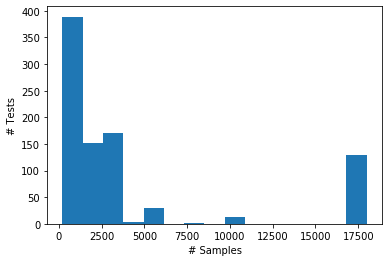
\includegraphics[width=\columnwidth]{Sections/test_lengths.png}
    \caption{Distribution of flight log lengths for the $N=888$ logs that were kept in the data set ($200 \leq l_k \leq 20000$)}
    \label{fig:test_lengths}
\end{figure}

As mentioned in \ref{data_set_properties} each datum is a multivariate time series with $n=10$ variables (listed in table~\ref{tab:in_outs}). 
During the data pre-processing, after the time series data is converted into tensors, all of the shorter $T_i$s were post-padded to the length of the longest one: $L=18001$ time steps. 

\section{Results}
Answers to research questions should come here


Maybe the traditional statistical CPD algorithms could outperform our method if they were boosted by feature engineering. But the feature engineering task is can become an arduous and inefficient task quickly. It exists so it compensates for inability of traditional methods to automatically find meaningful features from the data. \cite{bengio2013deep}



\begin{figure*}[ht]
    \centering
    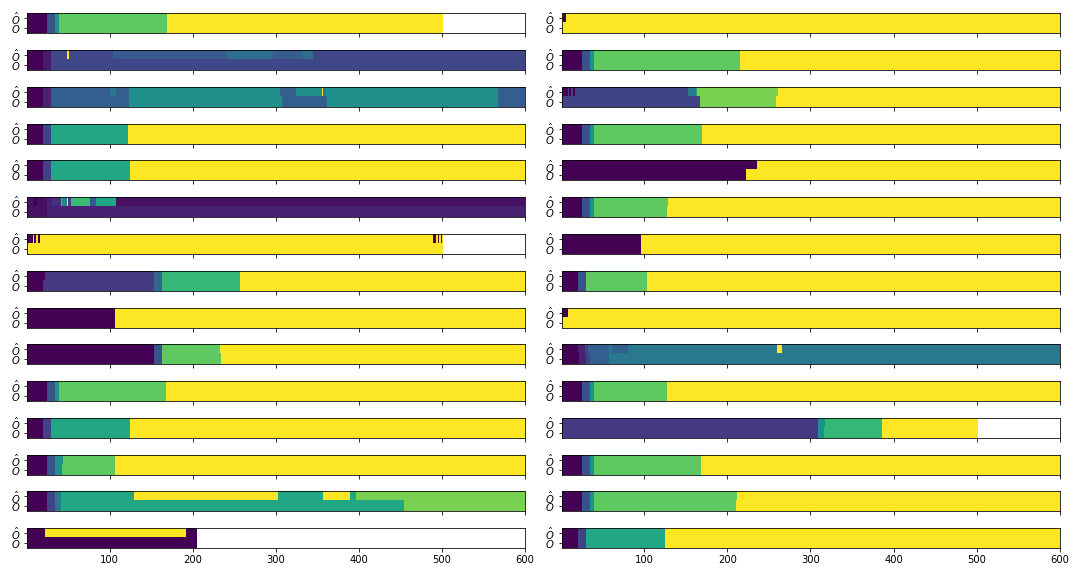
\includegraphics[width=\linewidth]{Sections/test_0.png}
    \caption{Evaluation of the model on unseen data. Each graph shows the state changes in one run of the system. The colors show the states. Top half of each plot depicts model's prediction of the system state ($\hat{O}$) and the bottom half shows the true labels($O$). Since the output is one-hot encoded, the item with the most probability is used as the predicted label at each point in time. X-axis is the time axis. Only the first 600 samples (2 minute of simulation) are shown to improve legibility.}
    \label{fig:test_0}
\end{figure*}
